\documentclass[]{beamer}
\usepackage[scale=1.15]{beamerposter} % use scale from 1.1 to 1.2

\usepackage{beamerposter}

\usetheme{vegaposter} 


\addbibresource{refs.bib}
\usepackage{lipsum}
 
\title{Monte-Carlo Pricing under the Heston Model}
\author{Artemy Sazonov, Danil Legenkiy, Kirill Korban}
\supervisor{Mikhail Zhitlukhin, Charles-Henri Roubinet}
\researchgroup{Stochastic Volatility Models}

\begin{document}
\nocite{*} % This is needed to make sure that all references are included in the bibliography

\begin{frame}[t]
    \begin{columns}[t] % The whole poster consists of three major columns, the second of which is split into two columns twice - the [t] option aligns each column's content to the top
     
    \begin{column}{\sepwid}\end{column} % Empty spacer column
    
    \begin{column}{\onecolwid} % The first column
     
    %----------------------------------------------------------------------------------------
    %	INTRODUCTION
    %----------------------------------------------------------------------------------------
    
    \begin{block}{Abstract}
        This paper uses Monte-Carlo simulations to evaluate the pricing of exotic options 
        under the Heston model. We apply the Euler-Maruyama scheme, along with the Andersen 
        Quadratic-Exponential and Andersen Truncated Gaussian schemes to perform the simulations.
        We compare the numerical precision of the simulated European call option prices with the 
        closed-form solutions from the Heston model. Our investigation of numerical experiments 
        reveal that the most efficient discretization scheme is the QE one.

        \
    \end{block}
    
    %----------------------------------------------------------------------------------------
    %	OBJECTIVES
    %----------------------------------------------------------------------------------------
    \vspace{1.in}

    \begin{alertblock}{Objectives}
    \begin{itemize}
    \item Implement the Numba/CUDA Euler and Andersen QE \& TG schemes;
    \item Implement the pricing interface;
    \item Implement the variance reduction methods;
    \item Compare the European call option prices from the \cite{Heston1993} and MC-simulated prices.
    \end{itemize}
    \end{alertblock}

    \vspace{1.in}
    
    
    %------------------------------------------------
    \begin{block}{Problem statement}
        The main problem with the Heston model is that there are only a few derivative and structural contract types for which the \emph{close-form prices} exist.
        Therefore, we need to think of a Monte-Carlo discretization method which is both computationally efficient and accurate enough.
        
        \

        The central motivation of this research: \emph{there exists a trade-off between the  efficiency and accuracy of a scheme}.
        Furthermore, we have no way to compare these two factors of the scheme for anything but the vanilla or digital European options.
        Once we establish the optimal scheme, we can use it to price the exotics.
    \end{block}


    %----------------------------------------------------------------------------------------
    
    \end{column} % End of the first column
    
    \begin{column}{\sepwid}\end{column} % Empty spacer column
    
    \begin{column}{\twocolwid} % Begin a column which is two columns wide (column 2)
    
    \begin{columns}[t,totalwidth=\twocolwid] % Split up the two columns wide column
    
    \begin{column}{\onecolwid}\vspace{-.6in} % The first column within column 2 (column 2.1)
    
    %----------------------------------------------------------------------------------------
    %	MATERIALS
    %----------------------------------------------------------------------------------------
    
    \begin{block}{Schemes}
    \textbf{Modified Euler Scheme}
    \begin{align}
        X_{n+1} & = X_n + (\mu - 0.5 v_n^+)h_n + \sqrt{v_n^+} \sqrt{h_n} Z_{1,n}, \label{Euler:Heston:price:posmod}\\
        v_{n+1} & = v_n + \kappa\left(\bar v - v_n^+\right) h_n + \gamma \sqrt{v_n^+} \sqrt{h_n} Z_{2,n}. \label{Euler:Heston:variance:posmod}
    \end{align}

    \textbf{Truncated Gaussian Scheme}
    \begin{equation}
        \left(\left.v_{n+1}\right| v_n\right) \overset{\text{law}}{=} \left(\mu(\Delta, v_n) + \sigma(\Delta, v_n) Z\right)^+,
    \end{equation}
    where $Z$ is a standard normal random variable and $\mu$ and $\sigma$ are the 'mean' and the 'standard deviation' of the desired distribution.
    
    \end{block}
    
    \
    
    %----------------------------------------------------------------------------------------
    
    \end{column} % End of column 2.1
    
    \begin{column}{\onecolwid}\vspace{-.6in} % The second column within column 2 (column 2.2)
    
    %----------------------------------------------------------------------------------------
    %	METHODS
    %----------------------------------------------------------------------------------------
    
    \begin{block}{Schemes}
    \textbf{Quadratic-Exponential Scheme}
    Let $\psi = \frac{m^2}{\sigma^2}$. 
    \begin{itemize}
        \item{$\psi > \psi_c$: } Quadratic case
        \begin{equation}
            \left(\left.v_{n+1}\right| v_n\right) \overset{\text{law}}{=} a(\Delta, v_n) \left(b(\Delta, v_n) + Z\right)^2;
        \end{equation}
        \item{$\psi \leq \psi_c$: } Exponential case
        \begin{multline}
            \P\left(\left. v_{n+1} \in [x, x+dx]\right|v_n\right) = \left(p(\Delta, v_n)\delta(0) \right.+\\\left.+ \beta(\Delta, v_n)(1-p(\Delta, v_n))e^{-\beta(\Delta, v_n) x}\right)dx.
        \end{multline}
    \end{itemize}
    \end{block}
    
    %----------------------------------------------------------------------------------------
    
    \end{column} % End of column 2.2
    
    \end{columns} % End of the split of column 2 - any content after this will now take up 2 columns width
    
    %----------------------------------------------------------------------------------------
    %	IMPORTANT RESULT
    %----------------------------------------------------------------------------------------
    
    \begin{figure}
        \label{fig:errors}
        \centering
        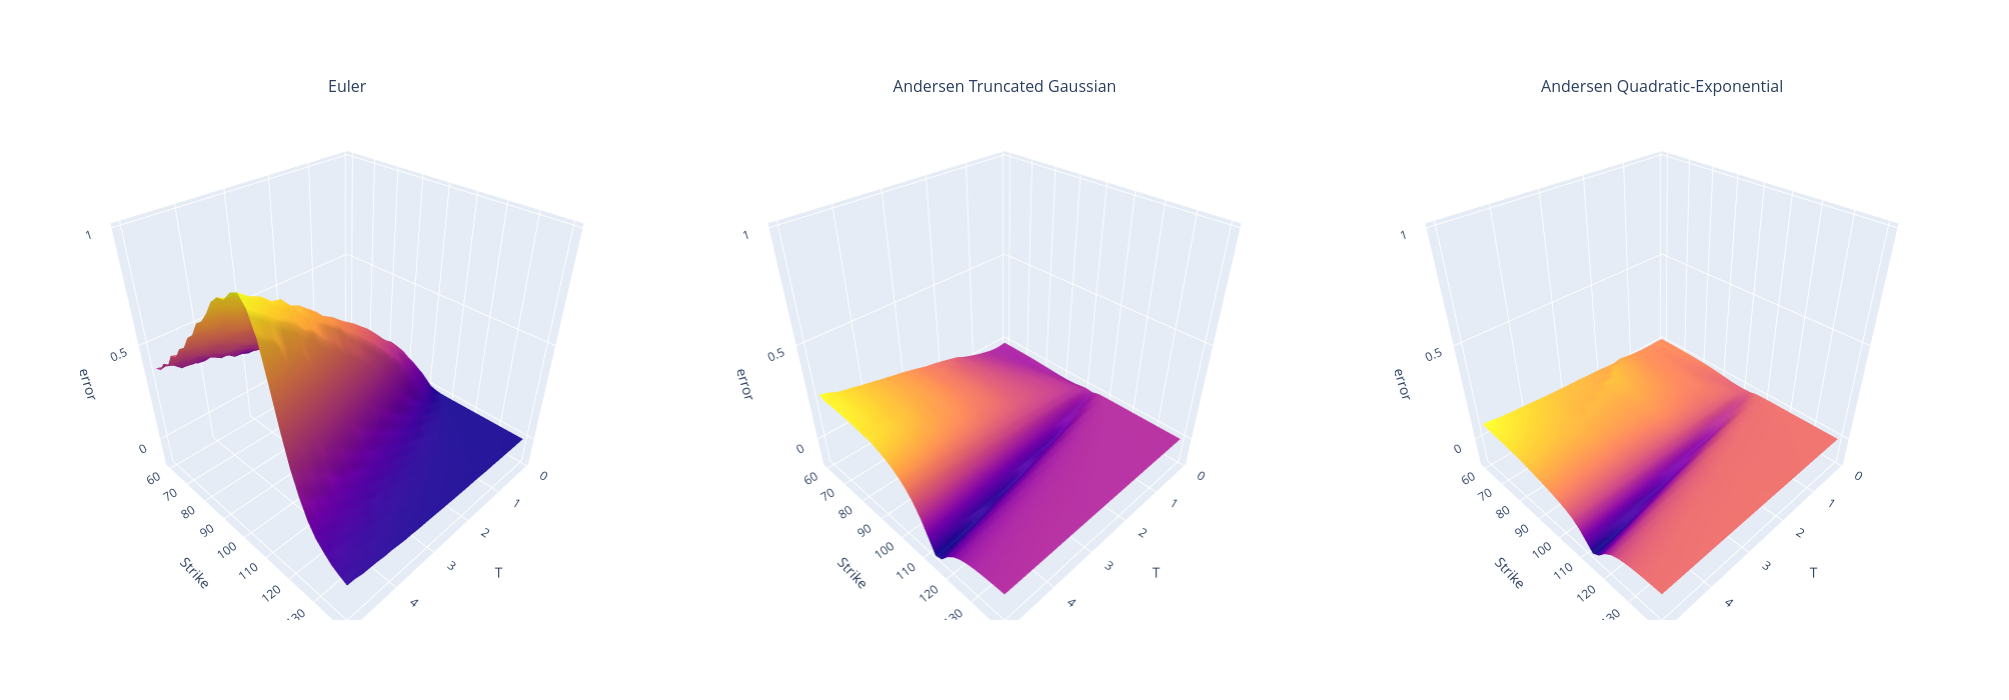
\includegraphics[width=\twocolwid]{figures/plot.png}
        \caption{Absolute errors of the schemes in the following order: Euler, TG, QE.}
    \end{figure}
    
    %----------------------------------------------------------------------------------------
    
    \begin{columns}[t,totalwidth=\twocolwid] % Split up the two columns wide column again
    
    \begin{column}{\onecolwid} % The first column within column 2 (column 2.1)
    
    %----------------------------------------------------------------------------------------
    %	MATHEMATICAL SECTION
    %----------------------------------------------------------------------------------------
    
    \begin{block}{Antithetic Variates}
        Suppose that we have two correlated identically distributed samples $Y^1$ and $Y^2$: $\cov[Y_i^1, Y_j^2] = \delta_{ij}\cov[Y_i^1, Y_i^2]$.
        Then we could introduce the following estimator:
        \begin{equation}
            \hat\theta_{\operatorname{AV}} = \frac{\bar Y^1 + \bar Y^2}{2}.
        \end{equation}
        Again, we can see that this estimator is unbiased and consistent. The variance of this estimator is
        \begin{equation*}
            \var \hat\theta_{\operatorname{AV}} = \frac{1}{4} \var[\bar Y^1] + \frac{1}{4} \var[\bar Y^2] + \frac{1}{2} \cov[\bar Y^1, \bar Y^2] .
        \end{equation*}
        Thus, the variance reduction effect takes place when $\rho < 0$. If $Y^1 = g(U)$, then its antithetic 
        variate is $Y^2 = g(1-U)$, where $U \sim U[0, 1]$. 
    \end{block}
    
    %----------------------------------------------------------------------------------------
    
    \end{column} % End of column 2.1
    
    \begin{column}{\onecolwid} % The second column within column 2 (column 2.2)
    
    %----------------------------------------------------------------------------------------
    %	RESULTS
    %----------------------------------------------------------------------------------------
    
    \begin{block}{Control Variates}
        Suppose that we have another random variable $Z$ that is correlated with $Y$ and 
        $\E\left[Z\right] = \mu$ is known. Then we could introduce the following estimator:
        \begin{equation}
            \hat\theta^b = \bar Y + b(\bar Z - \mu),
        \end{equation}
        where $b$ is a constant. Obviously, $\hat\theta^b$ is a consistent unbiased estimator of 
        $\theta$. How do we choose $b$? We need to minimize the variance of $\hat\theta^b$. A simple 
        unconstrained optimization problem:
        \begin{equation*}
            \var \hat\theta^b = \var \bar Y + b^2 \var \bar Z - 2b \cov [\bar Y, \bar Z] \to \min_b.
        \end{equation*}
        The solution is
        \begin{equation}
            b^* = \frac{\cov [Y, Z]}{\var Z}.\label{eq:control_variates:bopt}
        \end{equation}
    
    \end{block}
    
    %----------------------------------------------------------------------------------------
    
    \end{column} % End of column 2.2
    
    \end{columns} % End of the split of column 2
    
    \end{column} % End of the second column
    
    \begin{column}{\sepwid}\end{column} % Empty spacer column
    
    \begin{column}{\onecolwid} % The third column
    
    %----------------------------------------------------------------------------------------
    %	CONCLUSION
    %----------------------------------------------------------------------------------------
    
    \begin{block}{Results}
        \textbf{Accuracy and Performance}: Euler overprices the calls, QE and TG underprice the calls. See Fig. \ref*{fig:errors}. 
        \begin{table}
        \vspace{2ex}
        \begin{tabular}{c c c c}
            \hline
            \textbf{Scheme} & \textbf{N\_T} & \textbf{Time} & \textbf{Error}\\
            \hline
            Euler                 &      110      &    1.365      &    0.108692   \\\hline
            Truncated Gaussian    &      10       &    0.131      &    -0.077350  \\
            Truncated Gaussian    &      110      &    1.525      &    -0.002841  \\\hline
            Quadratic-Exponential &      10       &    0.139      &    -0.107819  \\
            Quadratic-Exponential &      110      &    1.590      &    -0.011618  \\
            \hline
            \
        \end{tabular}
        \caption{Accuracy-Performance comparison.}
        \end{table}

        \textbf{Antithetic Variates}
            
        For various combinations of both the Heston parameters and the discretization parameters, we
        have found that the variance reduction effect is approximately around 40\% when only 1 random variable has an antithetic one, and up to around 90\% for the AV estimator with 2 degrees of freedom.


        \textbf{Control Variates}
        
        We have found out that with the AV estimator with 2 degrees of freedom using the CV estimator speeds up the code by around 200\% (while pricing the Asian options).
    \end{block}
    
    \

    %----------------------------------------------------------------------------------------
    %	REFERENCES
    %----------------------------------------------------------------------------------------
    
    \begin{block}{References}
    
%    \nocite{*} % Insert publications even if they are not cited in the poster
    \printbibliography
    
    \end{block}
    
    \end{column} % End of the third column
    
    \begin{column}{\sepwid}\end{column} % Empty spacer column
    
    \end{columns} % End of all the columns in the poster
        
    \end{frame} % End of the enclosing frame
\end{document}